{\bf Изучение влияния параметра штрафной функции SVM классификатора.}
По-умолчанию, параметр рассматривается равным $1$. В подходе \cite{modernApproach}
такой параметр предварительно настраивался был равен $0.05$.
% !! Имеет смысл рассмотреть и при меньших параметрах.

В качестве данных для изучения выберем коллекции {\it SentiRuEval-2015} ввиду их
доступности на момент проведения аналогичных соревнований 2016 года. Для
обучения моделей выбраны сбалансированные коллекции, поскольку коллекции такого
типа и большего объема позволяют достичь наилучшего резульатата. На рисунке
\ref{fig:cost} приведены измененения результатов прогонов в зависимости от
величины параметра штрафной функции классификатора SVM.

\begin{figure}[!htp] \centering
    \captionsetup[subfigure]{justification=centering}
    \begin{subfigure}[b]{0.45\textwidth}
        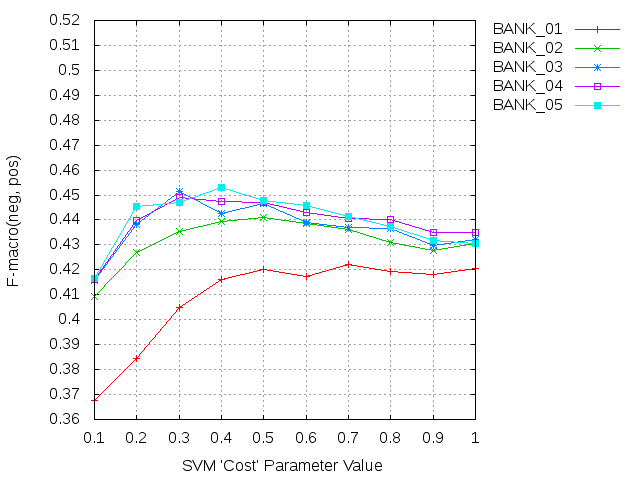
\includegraphics[width=\textwidth]{pics/2015_bank_balanced.png}
        \caption{BANK}
        \label{fig:bank_cost_changes}
    \end{subfigure}
    ~
    \begin{subfigure}[b]{0.45\textwidth}
        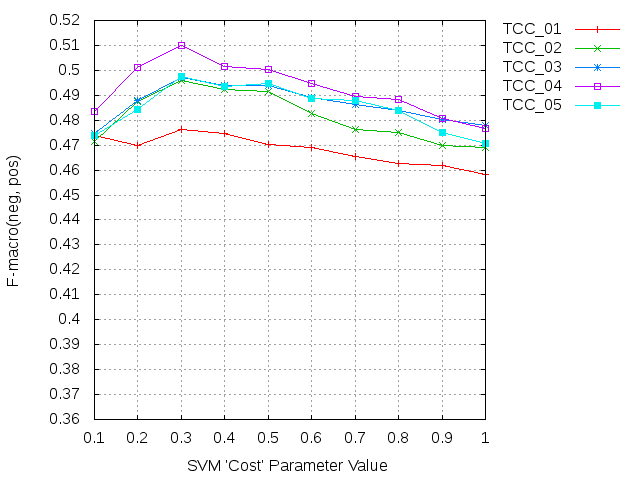
\includegraphics[width=\textwidth]{pics/2015_ttk_balanced.png}
        \caption{TCC}
        \label{fig:ttk_cost_changes}
    \end{subfigure}
    \caption{
        Влияние {\it параметра штрафной функции SVM классификатора}
        на результаты прогонов.
        Кривыми на графиках обозначается прогоны с соответсвующими номерами.
        Значение параметра измерялось в пределе $[0.1, 1]$ с шагом $0.1$.
    }
    \label{fig:cost}
\end{figure}

Основываясь на полученных результатах можно сделать вывод о проведении дальнейшего
тестирования на данных {\it SentiRuEval-2016}.
Для задачи BANK имеет смысл пересмотреть результаты при значении параметра в
диапазоне $[0.3, 0.5]$ (рис. \ref{fig:bank_cost_changes}).
Что касается задачи TCC, то здесь подходящим параметром явзяется значение в $0.3$
(рис. \ref{fig:ttk_cost_changes}).
